
\qquad
\pagestyle{empty}
\newpage


\chapter*{Introduction}

%\begin{flushright}
%\emph{Within a few years a simple and inexpensive device, readily carried about, will enable one to receive on land or sea the principal news, to hear a speech, a lecture, a song or play of a musical instrument, conveyed from any other region of the globe.}\\ -Nikola Tesla, 1905. 
%\end{flushright}
%\vspace*{0.6cm}

Since the early anatomical studies, the reproduction of images has been one of the main tool to investigate structures and differences of organs and organisms. 
Better ways to represent reality have undoubtedly led to better ways to understand it, and the work of pioneers in each of the discipline sharing the common need of precise and detailed images, were aided by available techniques offered in every epoch. 
\begin{figure}[!ht]
	\centering
	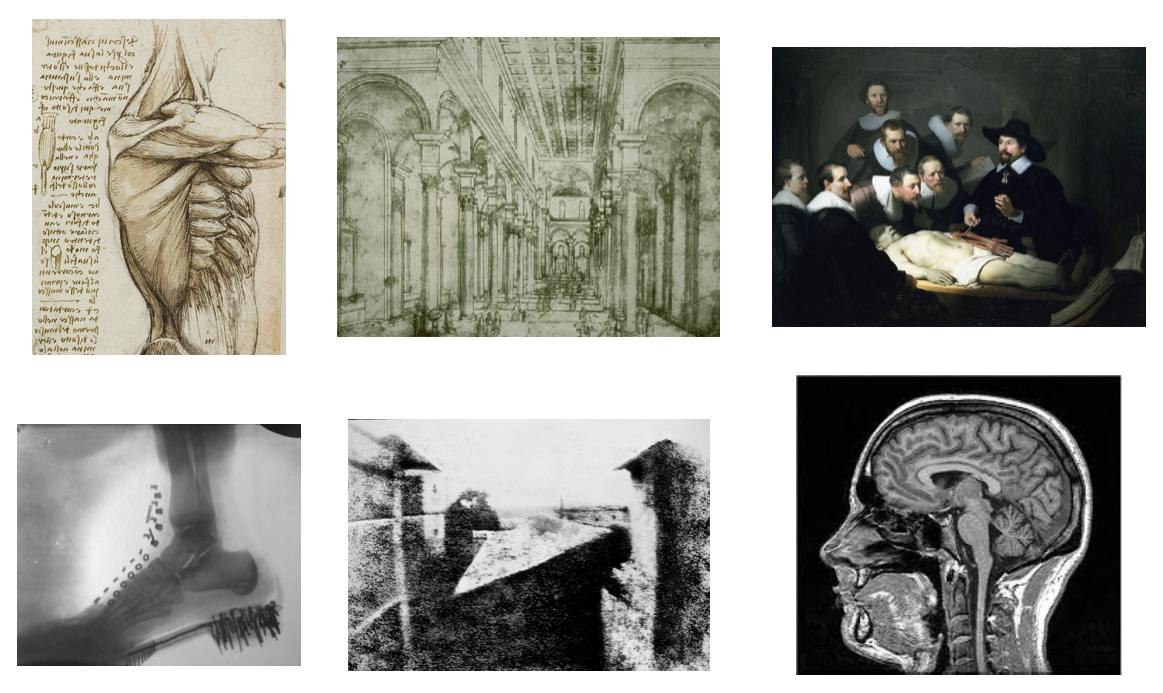
\includegraphics[scale=0.35]{figures/image_evolution.png}
	\label{fig:evolution}
\end{figure}  
At the dawn, Artists and Anatomists not surprisingly could have not be separated, and every enhancement made in one field followed immediately one in the other.
Although, whatever name every age gave to disciplines, the origin of every improvement in the field of images has its roots in the study of Geometry.\\
The first and most significant example is the powerful idea of perspective. Fixing a point from where to start infinitely parallel straight lines, leads, 16 centuries after their formalizations, Brunelleschi to revolutionize the  world's perception in artists' minds.
Two centuries later, when the inventors' work took the name of Science, the study of magnifying lenses and their combination, made available new explorable territories. Here again the Geometry couldn't have more important role in the systematic study of the lights deformation effect through conic-shaped glass.\\
Growing number of needs grows skills and techniques: artist, scientist and anatomist could not stay anymore below the same person's name, but what has remained constant is that every new discovery and the improvement in one field became an immediate advancement in others.
With the first stages of photographic techniques in the early '800, in parallel with the Young double slit experiment and its Fresnel interpretation, scientific community bring new attention to the shape of light. In late years of the same century the elegant Maxwell unification and its formalization by Heaviside determined the geometrical parameters of light. The discovery of X-ray by the first Nobel prize Roentgen and its refinement by Tesla is considered \cite{bradley2008history} the birth certificate of Medical Imaging. Domain destined to walk hand by hand with physics and engineering and to be eventually the most collaborative and crossing discipline ever seen with a great number of others evolving domain. The transition from pencil's scientists and painting's artists to photographic equipment that characterize this period didn't affected only this newborn branch. Instruments brings literally light on the severe limits of human eye capabilities: what was hidden reality become visible. \\
Just after the formalization of electric and magnetic field's shape, and the consequent mastery of electrical forces, discoveries of photoelectric effect opened new fields in the Physics of matter. Contemporary reformulation of diffusion processes, provided what will be angular theories in the construction of fundamental equipment for medical imaging.\\
In the wake of the third industrial revolution, electronic engineering, with its radio circuits, triods and valves destined to became transistor, provided each time better instrument to medical science where the acquisition and manipulation of patient images is a thriving theme. 
Thanks to philanthropic, scientific and economic interest gravitating around health care, the complicated interaction between sciences, physics and medicine get smoothed leading to achievement as radiography, ultrasound, thermography, magnetic resonance, optical fiber, nuclear medicine, confocal microscopy just to name a few. Technologies aimed to visualize the interior of a body always attained from several parts to reach their aims. \\
When photography get rid of photosensitive films to welcome digital sensors, images become stored in byte's grids with consequent powerful manipulation possibilities. The translation of acquired data from several sources not always or entirely compatible with the human sight to a suitable form meets new challenges.
Among the various possibility offered by image processing, two tools to reveal internal features and compare anatomies in images analysis are mostly utilized in medicine: segmentation and registration.
Both aimed to investigate patients' anatomies and physiologies, segmentation consists in the enhance contours, detect edges and to reveal hidden structure. Registration is the process of determining correspondences between one or more images acquired from patients scans.\\
This Master Thesis deals with diffeomorphic image registration and, letting aside dribs and drabs history of science, still a few words about the state of the art are needed to complete its introduction.

\section*{Toward a Solution of an Ill Posed Problem}
Dealing with image registration means searching for a solution to an ill posed problem: transformations between anatomies are not unique, and the impossibility of recover the spatial or temporal evolution of a anatomical transformation from temporally isolated images, makes any validation a difficult, if not impossible task. Among all of the possible voxelwise mapping that transform one image into another one, clinical interest may vary according to the requirements of each specific case\footnote{A recent survey in medical image registration can be found in \cite{Sotiras:survey:13}.}. \\
In brain imaging, for example, registration is performed to examine differences between subjects to distinguish healthy from sick patients and for a better understanding of the disease's feature. Another case may require to compare different acquisition of the same subject, before and after a surgery or after a fixed period of time: parameters and features of the transformation are completely different. Also the correction of motion distortion in image's acquisition phase, the mosaicing of several images or the construction of the model of cardiac and respiratory motion may require customized image registration techniques.\\
Any approach is therefore varied and flexible: this led to a wide range of tools that has been proposed by researchers in the last decades\footnote{A quick glance to Google scholar reveals about $1200000$ papers in \emph{medical image registration} (55\% of the whole \emph{image registration} resources).}.\\
There are several features that distinguish image registration's algorithm, but the most relevant is the choice of the family to whom the transformation belongs. Since anatomies appears to transform continuously over time, without any variation in the topological features, the use of diffeomorphisms as transformation appears one of the most natural.\\
The continuous nature of these functions appears to be in contrast with the discrete nature of voxel images as well as with any computer's parametrization ability.\\
The approach of modeling with richer structure for simpler elements is actually very common even in less sophisticated math: for example when measuring the diagonal of a $1$ meters side table. The decimal unlimited non periodical $\sqrt{2}$ doesn't help until we don't consider it as an answer belonging to a larger-than-reality mathematical structure: computations and theorem (as the Pythagorean theorem) are well defined and meaningful.\\ 
Back to images, the simple structure of a raster image as 3-dimensional matrix is really limited if compared to the continuous object they represent. Modeling with continuous function provides a structure that reflects the object's topology. In addition enable us to apply mathematical features from differential geometry and dynamical system theory.\\
The first idea of using smooth and continuous function for image registration goes back to the idea of using the Navier-Cauchy partial differential equation to model the deformation of images as two balancing forces applied to an elastic body \cite{Broit:1981}. The solution's domain restriction to diffeomorphisms for the solution of the Lagrange transport equation for medical imaging registration appears in \cite{Dupuis:98:variationalproblems} and \cite{Trouve:98}, and with his many variants is an active subject of study for research in mathematic applied to medical imaging.
An important framework for the computation of image registration of diffeomorphism is provided by the Large Deformation Diffeomorphic Metric Mapping (LDDMM). Here diffeomorphisms are parametrized as ending point of integral curves of vector field on the Lie group of diffeomoprhism equipped with a Riemannian metric \cite{dupuis1998variational}, \cite{beg2005computing}. Solid mathematical foundations are payed in term of computational complexity. Different parametrization of diffeomorphisms, as Stationary Velocity Fields \cite{arsigny2006statistics} has been embedded in the LDDMM framework, to reduce computational time. This approach gives birth to the DARTEL \cite{Ashburner:07} and the Stationary LDDMM \cite{hernandez2007registration}. Starting from the Tririon's DEMON algorithm \cite{thirion1998image}, a different framework for diffeomorphic image registration was presented as Diffeomorphic Daemon \cite{vercauteren2007non} and the LCC-daemon \cite{lorenzi2013lcc} . A comparison between stationary LDDMM and Diffeomorphic Demons with emphasis in both theoretical and practical aspects can be found in \cite{hernandez2008comparing}. \\
The theme of diffeomorphism do not recurs only in medical application but it is a continuously improved subject of research also theoretical studies as \cite{Milnor:84:remarks}, \cite{bauer2011geodesic}, \cite{bauer2010sobolev} or studies applied to other domain of science \cite{Arnold:Khesin:14} \cite{ovsienko1992integrals}. Geometry remains an important underpinning structure for many achievement in medical imaging and still advanced research in geometry is actively used by this one.\\
Image registration do not involves only the construction of a transformation. The necessity of having statistics to infer the variability of anatomical structure bring the field of Patter Analysis from Machine Vision to Medical Imaging, with the name of Computational Anatomy (cite survey computational anatomy). 
Statistics on diffeomorphisms are naturally introduced relying on Lie algebras and introducing the log-euclidean framework; proposed for the first time in 2004 \cite{Arsigny:MRM:06} followed by an update of 2006 , as a faster improvement to the affine invariant Riemannian approach. It has found successful applications in many domains of medical imaging (in vivo mosaicing \cite{Vercauteren:PHD:08}, brain Alzheimer detection \cite{Lorenzi:PhD:12}, cardiac image analysis \cite{Mansi:IJCV:11}, mandible imaging using polyaffine registration \cite{Seiler:MICCAI:11}) and has been continuously improved.\\
Sono quindi molteplici le facce da studiare e dalle quali attingere che l'uso dei diffeomorfismi comporta: 

la ricerca teorica, il loro uso nelle applciazioni pratiche e il loro sudio nell'analisti statistica dell'evoluzione delle deformazioni anatomiche. 

Aim of this thesis is to present numerical methods to compute the composition fo diffeomorphisms in the log-euclidean framework. 
Questa tesi sviluppa il tema particolare della loro composizione, usando lo sviluppo in serie di taylor, le accelerazioni delle serie numeriche, e il parallel transport, tantando di tenere conto degli aspetti teorici e pratici della questione.
 


% % % % % % % % % % % % % % % % % % % % % % % % % % % % % % % % % % % % % %
% % SUB SECTION
% % % % % % % % % % % % % % % % % % % % % % % % % % % % % % % % % % % % % %
\section*{Thesis' Organization and No(ta)tions}

The first chapter about the general framework in image registration and parametrization of diffeomorphisms for LDDMM and SVF is followed by three distinct part. The first one presents basic tools of differential geometry and parallel transport, with emphasis on the computational side. The second part is about the principal objects utilized to explore new numerical techniques and to compare them with the one currently utilized. The last part is devoted to the results for the computation on synthetic dataset and on patient images. \\

\begin{enumerate}
	\item[{\bf Chapter \ref{se:registration_framework}:}] introduction of the registration framework. After a first section about the main definitions and concept used throughout the thesis, we present the main feature of the general framework used to perform registration. Particular attention is given to the pros ad cons of using diffeomorphism as set of transformation between anatomies and some considerations about the current methods currently used for the implementation: the LDDMM and SVF. 
	
	\item[{\bf Chapter \ref{ch:finite_lie_group}:}] an in deep of the possibilities of set of transformations when provided by mathematical structure of Lie group. Main mathematical elements and tools from Lie group theory directly involved in the image registration techniques are formally defined with a particular attention to flows, left translation, push forward, Lie logarithm and Lie exponential. We define as well the concept of Log-composition around which the research gravitates: it originates form the BCH formula, presented here as well as the first more immediate way to compute the Log-composition. The second way to compute it is provided by the Taylor expansion, presented in the last section.
	
	\item[{\bf Chapter \ref{ch:parallel_transport}:}] BCH and Taylor expansion are tow possibility to compute the Log-composition. A third one presented in this chapter originates by a geometrical approach and it is given by the parallel transport. The first and the second sections are devoted to present the theoretical tools to define formally the parallel transport. Last section is about two strategies to compute the parallel transport without involving the Christoffel symbols: the Schild's Ladder and the Pole Ladder.
	
	\item[{\bf Chapter \ref{ch:accelerating}:}] ...
	
	\item[{\bf Chapter \ref{ch:rigid_body_transformations} and \ref{ch:svf}:}] validity of results in the Log-composition computation are tested with two groups of transformations commonly used in medical image registration: the group of rigid body transformation and the group of diffeomorphisms (expressed in the application as the set of Stationary Velocity Fields). These chapters are aimed to present them in details and they are oriented to the application. 
	
	
    \item[{\bf Chapter \ref{ch:application_log_composition}:}] this is the central part of the research. The Log-composition is analyzed as s valuable tool in image registration, within the framework presented in chapter \ref{se:registration_framework}. A summary of the methods for its computation is presented as possible numerical approximation to be utilized for image registration: BCH formula, Taylor expansion, parallel transport and Accelerating Convergences series. 
    
    
     \item[{\bf Chapter \ref{ch:lie_log_computation}:}]  the algorithm for the Lie-logarithm computation presented in \emph{A new algorithm for the computation of the group logarithm of diffeomorphism} \cite{Bossa:08} gravitates around the BCH formula. If reformulated with the Log-composition each of its numerical approximation is a valid tool to improve its performance. Of particular interests are the methods that avoid the computation of the BCH formula on which the algorithm was initially based.
     
	\item[{\bf Chapter \ref{ch:results}:}] is devoted to experimental results. Performance of the Log-composition applied to rigid body transformation and diffeomorphisms are separately computed and compared. In addition a version of NiftyReg based on various we present the results of the numerical methods presented in the previous section, on synthetic data as well as on clinical data within a version of the  LCC-Demons customized with parallel transport.
	
	
	\item[{\bf Chapter \ref{ch:conclusions}}] we draw the conclusion of what has been done so far (with a shameless and challenging emphasis of what is missing and what is still to be done).

	
	
\end{enumerate}








